%%\title{Local Reference System}
%  Changed by: Chris ISELIN, 17-Jul-1997 

%  Changed by: Hans Grote, 25-Sep-2002 

%%\usepackage{hyperref}
% commands generated by html2latex


%%\begin{document}
%%\begin{center}
 %%EUROPEAN ORGANIZATION FOR NUCLEAR RESEARCH 
%%\includegraphics{http://cern.ch/madx/icons/mx7_25.gif}

\subsection{Local Reference Systems}
%%\end{center}

\subsection{\href{straight}{Reference System for Straight Beam Elements}} In straight elements the local reference system is simply translated by the length of the element along the local \textit{s}-axis. This is true for 
\begin{itemize}
	\item \href{drift.html}{Drift space}, 
	\item \href{quadrupole.html}{Quadrupole}, 
	\item \href{sextupole.html}{Sextupole}, 
	\item \href{octupole.html}{Octupole}, 
	\item \href{solenoid.html}{Solenoid}, 
	\item \href{crabcavity.html}{CRABCAVITY}, 
	\item \href{cavity.html}{RF cavity}, 
	\item \href{separator.html}{Electrostatic separator}, 
	\item \href{kickers.html}{Closed orbit corrector}, 
	\item \href{monitors.html}{Beam position monitor}. 
\end{itemize} The corresponding \textit{R}, \textit{S} are 


%%\includegraphics{null}
%RSstraight
\[
R =
 \begin{pmatrix}
  0 \\
  0 \\
  L
 \end{pmatrix}
, \quad
S =
 \begin{pmatrix}
  1 & 0 &  0 \\
  0 & 1 &  0 \\
  0 & 0 &  1
 \end{pmatrix}
.
\]

 A rotation of the element about the \textit{S}-axis has no effect on \textit{R} and \textit{S}, since the rotations of the reference system  before and after the element cancel. 
%%\begin{center}

%%\includegraphics{null}
\begin{figure}[H]
  \centering
	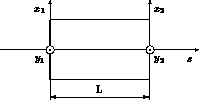
\includegraphics{figures/ref_straight.png}
  \caption{Reference System for Straight Beam Elements}
%\\\textbf{Figure 1:} Reference System for Straight Beam Elements 
\end{figure}


\subsection{\href{rbend}{Reference System for Bending Magnets}}\href{bend.html}{Bending magnets} have a curved reference orbit. For both rectangular and sector bending magnets 


%%\includegraphics{null}
%RSbend
\[
R =
 \begin{pmatrix}
  \rho\,(\cos \alpha - 1) \\
  0 \\
  \rho\,\sin \alpha
 \end{pmatrix}
, \quad
S =
 \begin{pmatrix}
  \cos \alpha & 0 &  -\sin \alpha \\
  0 & 1 &  0 \\
  \sin \alpha & 0 &  \cos \alpha
 \end{pmatrix}
,
\]

 where alphais the bend angle. A positive bend angle represents a bend to the right, i.e. towards negative \textit{x} values. For sector bending magnets, the bend radius is given by rho, and for rectangular bending magnets it has the value 

 rho = \textit{L} / 2 sin(alpha/2). 

 If the magnet is rotated about the \textit{s}-axis by an angle psi, \textit{R} and \textit{S} are transformed by 

\textit{R}* = \textit{T R}, \textit{S}* = \textit{T S T$^-1$}. 

 where \textit{T} is the orthogonal rotation matrix 


%%\includegraphics{null}
%Trot
\[
T =
 \begin{pmatrix}
  \cos \psi &  -\sin \psi & 0 \\
  \sin \psi &  \cos \psi & 0 \\
	0			&	0			 & 1 
 \end{pmatrix}
.
\]

 The special value psi = pi/2 represents a bend down.  
%%\begin{center}
%\href{rbend}{
%%%\includegraphics{null}}
\begin{figure}[H]
  \centering
	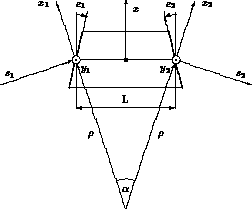
\includegraphics{figures/ref_rbend.png}
  \caption{Reference System for Rectangular Bends; The signs of the pole-face rotations are positive as shown.}
%\\\textbf{Figure 2:} Reference System for Rectangular Bends; The signs of the pole-face rotations are positive as shown. 
\end{figure}

%%\includegraphics{null}}
\begin{figure}[H]
  \centering
	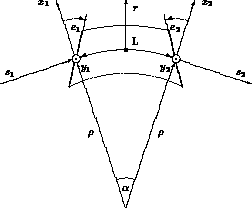
\includegraphics{figures/ref_sbend.png}
  \caption{Reference System for Sector Bends; The signs of the pole-face rotations are positive as shown. }
%\\\textbf{Figure 3:}  Reference System for Sector Bends; The signs of the pole-face rotations are positive as shown. 
\end{figure}


\subsection{Elements which do not Change the Local Reference}\href{marker.html}{MARKER} elements do not  affect the reference orbit. They are ignored for geometry calculations.  

\href{http://www.cern.ch/Hans.Grote/hansg_sign.html}{hansg}, January 24, 1997 

%%\end{document}

% add other files to the end of this file

%%%\title{DRIFT}
%  Changed by: Chris ISELIN, 24-Jan-1997 
%  Changed by: Hans Grote, 30-Sep-2002 

\section{Drift Space}

\begin{verbatim}
label: DRIFT,L=real;
\end{verbatim} 

A DRIFT space has one real attribute: 
\begin{itemize}
   \item L: The drift length (default: 0 m) 
\end{itemize} 

Examples: 
\begin{verbatim}
DR1: DRIFT, L = 1.5;
DR2: DRIFT, L = DR1[L];
\end{verbatim} 

The length of DR2 will always be equal to the length of DR1. The
\href{../Introduction/local_system.html#straight}{straight  reference
  system} for a drift space is a cartesian coordinate system.  

%\href{http://www.cern.ch/Hans.Grote/hansg_sign.html}{hansg}, January 24, 1997 

%%%\title{QUADRUPOLE}
%  Changed by: Chris ISELIN, 27-Jan-1997 
%  Changed by: Hans Grote, 30-Sep-2002 
%  Changed by: Frank Schmidt, 28-Aug-2003 
%  Changed by: Andrea Latina, 6-May-2013 

\section{Quadrupole}

\begin{verbatim}
label: QUADRUPOLE, L = real, K1 = real, K1S = real, TILT = real;
\end{verbatim}    

A QUADRUPOLE has four real attributes:     
\begin{itemize}
   \item L: The quadrupole length (default: 0 m). 
   \item K1: The normal quadrupole coefficient \\        
     \textit{K}$_1$ = 1/(\textit{B} rho) ($\partial$\textit{B$_y$}/$\partial$\textit{x}).\\ 
     The default is 0 m**(-2). A positive normal quadrupole strength
     implies horizontal focussing of positively charged particles.  
   \item K1S: The skew quadrupole coefficient \\        
     \textit{K}$_{1s}$ = 1/(2 \textit{B} rho)
     ($\partial$\textit{B$_x$}/$\partial$\textit{x} -
     $\partial$\textit{B$_y$}/$\partial$\textit{y})\\  
     where (x,y) is now a coordinate system rotated by -45$^o$ around s
     with respect to the normal one. The default is 0  m**(-2). A
     positive skew quadrupole strength implies defocussing (!) of
     positively charged particles in the (x,s) plane rotated by 45$^o$
     around s (particles in this plane have x = y $>$ 0). 
   \item TILT: The roll angle about the longitudinal axis (default: 0
     rad, i.e. a normal quadrupole). A positive angle represents a
     clockwise rotation. A TILT=pi/4 turns a positive normal quadrupole
     into a negative skew quadrupole.          

\textbf{ Please note that contrary to MAD8 one has to
  specify the desired TILT angle, otherwise it is taken as
  0 rad. This was needed to avoid the confusion in MAD8
  about the actual meaning of the TILT attribute for
  various elements. } 

    \item THICK: If this flag is set to 1 the quadrupole will be tracked
      through as a thick-element, instead of being converted into
      thin-lenses.  
\end{itemize}

\textbf{ Note also that K$_1$/K$_{1s}$ can be considered as
  the normal or skew quadrupole components of the magnet on
  the bench, while the TILT attribute can be considered as an
  tilt alignment error in the machine. In fact, a positive
  K$_1$ with a tilt=0 is equivalent to a positive K$_{1s}$
  with positive tilt=+pi/4. } 

Example: 
\begin{verbatim}
QF: QUADRUPOLE, L = 1.5, K1 = 0.001, THICK = 1;
\end{verbatim}     

The \href{local_system.html#straight}{straight reference system} for
a quadrupole is a cartesian coordinate system.

%\href{http://www.cern.ch/Hans.Grote/hansg_sign.html}{hansg},
%\href{http://www.cern.ch/Frank.Schmidt/frs_sign.html}{frs},
%\href{https://phonebook.cern.ch/phonebook/?id=PE525753}{al},       May 6, 2013 

%%%\title{SEXTUPOLE}
%  Changed by: Chris ISELIN, 27-Jan-1997 

%  Changed by: Hans Grote, 30-Sep-2002 

%  Changed by: Frank Schmidt, 28-Aug-2003 

%%\usepackage{hyperref}
% commands generated by html2latex


%%\begin{document}
%%\begin{center}
 %%EUROPEAN ORGANIZATION FOR NUCLEAR RESEARCH 
%%\includegraphics{http://cern.ch/madx/icons/mx7_25.gif}

\subsection{Sextupole}
%%\end{center}
\begin{verbatim}

label: SEXTUPOLE,L=real,K2=real,K2S=real,TILT=real;
\end{verbatim} A SEXTUPOLE has four real attributes: 
\begin{itemize}
	\item L: The sextupole length (default: 0 m). 
	\item K2: The normal sextupole coefficient 

\textit{K}$_2$ = 1/(\textit{B} rho) ($\partial$$^2$\textit{B$_y$}/$\partial$ \textit{x}$^2$). 

 (default: 0 m**(-3)). 
	\item K2S: The skew sextupole coefficient 

\textit{K}$_{2S}$ = 1/(2 \textit{B} rho) ($\partial$$^2$\textit{B$_x$}/$\partial$ \textit{x}$^2$ - $\partial$$^2$\textit{B$_y$}/$\partial$ \textit{y}$^2$). 

 where (x,y) is now a coordinate system rotated by -30$^o$ around s with respect to the normal one. (default: 0 m**(-3)). A positive skew sextupole strength implies defocussing (!) of positively charged particles in the (x,s) plane rotated by 30$^o$ around s (particles in this plane have x $>$ 0, y $>$ 0). 


	\item TILT: The roll angle about the longitudinal axis (default: 0 rad, i.e. a normal sextupole). A positive angle represents a clockwise rotation. A TILT=pi/6 turns a positive normal sextupole into a negative skew sextupole. 

\textbf{  Please note that contrary to MAD8 one has to specify the desired TILT angle, otherwise it is taken as 0 rad. This was needed to avoid the confusion in MAD8 about the actual meaning of the TILT attribute for various elements. }
\end{itemize}

\textbf{  Note also that K$_2$/K$_{2s}$ can be considered as the normal or skew sextupole components of the magnet on the bench, while the TILT attribute can be considered as an tilt alignment error in the machine. In fact, a positive K$_2$ with a tilt=0 is equivalent to a positive K$_{2s}$ with positive tilt=+pi/6.  }

Example: 
\begin{verbatim}

S: SEXTUPOLE,L=0.4,K2=0.00134;
\end{verbatim} The \href{local_system.html#straight}{straight reference system} for a sextupole is a cartesian coordinate system.  

\href{http://www.cern.ch/Hans.Grote/hansg_sign.html}{hansg}, \href{http://www.cern.ch/Frank.Schmidt/frs_sign.html}{frs}, August 28, 2003  

%%\end{document}

%%%\title{the mad program}
%  Changed by: Chris ISELIN, 27-Jan-1997 
%  Changed by: Hans Grote, 30-Sep-2002 
%  Changed by: Frank Schmidt, 28-Aug-2003 

\section{Octupole}

\begin{verbatim}
label: OCTUPOLE, L = real, K3 = real, K3S = real, TILT = real;
\end{verbatim} 

An OCTUPOLE has four real attributes: 
\begin{itemize}
   \item L: The octupole length (default: 0 m). 

   \item K3: The normal octupole coefficient \\
     \textit{K}$_3$ = 1/(\textit{B} rho)
     ($\partial$$^3$\textit{B$_y$}/$\partial$\textit{x}$^3$). \\ 
     (default: 0 m**(-4)). 

   \item K3S: The skew octupole coefficient 
%% 2013-Jul-05  18:00:59  ghislain: to be checked wrt error reported on
%% K2S for sextupoles 
     \textit{K}$_3S$ = 1/(2 \textit{B} rho)
     ($\partial$$^3$\textit{B$_x$}/$\partial$\textit{x}$^3$ -
     $\partial$$^3$\textit{B$_y$}/$\partial$\textit{y}$^3$). \\
     where (x,y) is now a coordinate system rotated by -22.5$^o$ around
     s with respect to the normal one. (default: 0 m**(-4)). A positive
     skew octupole strength implies defocussing (!) of positively
     charged particles in the (x,s) plane rotated by 22.5$^o$ around s
     (particles in this plane have x $>$ 0, y $>$ 0).  

   \item TILT: The roll angle about the longitudinal axis (default: 0
     rad, i.e. a normal octupole). A positive angle represents a
     clockwise rotation. A TILT=pi/8 turns a positive normal octupole
     into a negative skew octupole.  

     \textbf{  Please note that contrary to MAD8 one has to specify the
       desired TILT angle, otherwise it is taken as 0 rad. This was
       needed to avoid the confusion in MAD8 about the actual meaning of
       the TILT attribute for various elements. }

\end{itemize}

\textbf{  Note also that K$_3$/K$_3s$ can be considered as the normal or
  skew quadrupole components of the magnet on the bench, while the TILT
  attribute can be considered as an tilt alignment error in the
  machine. In fact, a positive K$_3$ with a tilt=0 is equivalent to a
  positive K$_3s$ with positive tilt=+pi/8. } 

Example: 
\begin{verbatim}
O3: OCTUPOLE, L = 0.3, K3 = 0.543;
\end{verbatim} 

The \href{local_system.html#straight}{straight reference system} for a
octupole is a cartesian coordinate system. Octupoles are normally
treated as thin lenses, except when tracking by Lie-algebraic methods.   

%\href{http://www.cern.ch/Hans.Grote/hansg_sign.html}{hansg}, 
%\href{http://www.cern.ch/Frank.Schmidt/frs_sign.html}{frs}, August 28, 2003  

%%%\title{SOLENOID}
%  Changed by: Chris ISELIN, 27-Jan-1997 
%  Changed by: Hans Grote, 30-Sep-2002 
%  Changed by: Alexander Koschik, 16-May-2006 

\section{Solenoid}

\texttt{label: SOLENOID, L = real, KS = real;           } (\textbf{thick} version) 
\\
\texttt{label: SOLENOID, L = 0,    KS = real, KSI=real; } (\textbf{thin} version) 

A SOLENOID has two or three real attributes: 
\begin{itemize}
   \item L: The length of the solenoid (default: 0 m) 
   \item KS: The solenoid strength \textit{K$_s$} (default: 0
     rad/m). For positive KS and positive particle charge, the solenoid
     field points in the direction of increasing \textit{s}.  
   \item KSI: The solenoid integrated strength \textit{K$_s$*L}
     (default: 0 rad).  This additional attribute is needed only when
     using the thin solenoid,  where \textit{L=0}!     
   \item \textit{ KNL \& KSL:  Take note that one can specify multipole
     coefficients but they have no effect in MAD-X proper but are used
     for solenoids with multipoles in PTC.} 
\end{itemize}

Example: 
\begin{verbatim}
SOLO: SOLENOID, L = 2., KS = 0.001;
THINSOLO: SOLENOID, L = 0, KS = 0.001, KSI = 0.002;
\end{verbatim}

The \href{local_system.html#straight}{straight reference system} for a
solenoid is a cartesian coordinate system. 
 
%\href{http://www.cern.ch/Hans.Grote/hansg_sign.html}{hansg}, January 27, 1977 

%%%\title{CRABCAVITY}
%  Added by: R. Calaga, Sep 2010 
%  Edited by: A. Latina, Jun 2013

\section{Crab Cavity}


\begin{verbatim}
label: CRABCAVITY, L = real, VOLT = real, LAG = real, FREQ = real,
                   RV1 = integer, RV2 = integer, RV3 = integer, RV4 = integer, 
                   RPH1 = integer, RPH2 = integer, 
                   LAGF = real, HARMON = integer;                 
\end{verbatim} 

%  BETRF=real, PG=real,
%  FREQ=real, SHUNT=real, TFILL=real; 

A CRABCAVITY has five real attributes and seven integer attributes: 

\begin{itemize}
  \item L: The length of the cavity (default: 0 m) 

  \item VOLT: The peak RF voltage (default: 0 MV). 

  \item LAG: The initial phase lag [2pi] (default: 0). 

  \item FREQ: The RF frequency [MHz] (no default). \\
    {\bf Note that if the RF frequency is not given, it is computed from the
    harmonic number and the revolution frequency \textit{f$_0$} as before. 
    However, for deflecting structures this makes no sense, and the 
    frequency is mandatory.} 

  \item RV1: Number of initial turns with zero voltage (default: 0). 
  \item RV2: Number of turns to ramp voltage from zero to nominal value (default: 0). 
  \item RV3: Number of turns with nominal voltage (default: 0). 
  \item RV4: Number of turns to ramp voltage from nominal value to zero (default: 0).  

  \item LAGF: Value of the final crab RF phase lag [2pi] (default: 0).

  \item RPH1: Number of initial turns with nominal phase (default: 0). 
  \item RPH2: Number of turns to ramp phase [2pi] from nominal to
    specified value \\ (default:~0). 

  \item HARMON: The harmonic number \textit{h} (no default). \\
    Only if the frequency is not given. 

% \item BETRF: RF coupling factor (default: 0).
% \item PG: The RF power per cavity (default: 0 MW).
% \item SHUNT: The relative shunt impedance (default: 0 MOhm/m).
% \item TFILL: The filling time of the cavity T<sub>fill</sub> (default: 0 microseconds). 
%\item EPHASE: Value of the final crab RF phase [2pi] with respect to  nominal value (default: 0). 
\end{itemize}


{\bf Caveats:}
\begin{itemize}
   \item \textit{ Please take note, that the following MAD8 attributes:
     BETRF, PG, SHUNT and TFILL are currently not implemented in MAD-X!}
   \item \textit{ Note that crab cavities are only implemented for
     tracking  purposes. \\ TWISS will ignore any effect of the crab cavity.  
% as well that twiss is 4D only. As a consequence the TWISS
% parameters in the plane of non-zero dispersion may not close as
% expected. Therefore, it is best to perform TWISS in 4D only, i.e. with
% cavities switched off. If 6D is needed one has to use the
% 
% <a href="../ptc_twiss/ptc_twiss.html">ptc_twiss</a> command. 
}
\end{itemize} 

%A cavity requires the particle energy (\href{beam.html#energy}{ENERGY})
%and the particle charge (\href{beam.html#charge}{CHARGE}) to be set by
%a \href{beam.html}{BEAM} command before any calculation is performed. 

Before any calculation is performed with a CRABCAVITY, the particle
energy (\href{beam.html#energy}{ENERGY}) and the particle charge
(\href{beam.html#charge}{CHARGE}) must be set by a
\href{beam.html}{BEAM} command.   

Then the effect of the CRABCAVITY on particle coordinates during tracking is
\\
\\ delta(\textit{px})  = VOLT * sin( PHI - OMEGA * t) 
\\ delta(\textit{E})  = -  VOLT * OMEGA * x * cos(PHI - OMEGA * t) 
\\ 
\\ where PHI =  2 $\pi$ * (LAG - HARMON * \textit{f$_0$ t}), 
\\ and OMEGA = 2 $\pi$ * FREQ / \textit{c}
\\
% delta(<i>E</i>) = VOLT * 
% sin(2 pi * (LAG - HARMON * <i>f<sub>0</sub> t</i>)). 


Example: 
\begin{verbatim}
BEAM, PARTICLE = PROTON, ENERGY = 7000.0;
CAVITY:  CRABCAVITY, L = 10.0, VOLT = 5.0, LAG = 0.0, FREQ = 400,
         RV1 = 0, RV2 = 50, RV3 = 1000, RV4 = 50, 
         RPH1 = 100, RPH2 = 500, LAGF = 0.125;
\end{verbatim} 

The \href{local_system.html#straight}{straight reference system} for a
cavity is a cartesian coordinate system.  
 
%\href{http://www.cern.ch/rcalaga}{R. Calaga}, September 2010

%%%\title{RFCAVITY}
%  Changed by: Chris ISELIN, 27-Jan-1997 
%  Changed by: Hans Grote, 30-Sep-2002 

\section{RF Cavity}


\begin{verbatim}
label: RFCAVITY, L = real, VOLT = real, LAG = real, HARMON = integer, FREQ = real;                  
\end{verbatim} 

%  HARMON=integer, BETRF=real,PG=real,
%                  FREQ=real,SHUNT=real,TFILL=real; 


An RFCAVITY has eight real attributes and one integer attribute: 
\begin{itemize}
   \item L: The length of the cavity (DEFAULT: 0 m) 
   \item VOLT: The peak RF voltage (DEFAULT: 0 MV). The effect of the cavity is \\
     delta(\textit{E}) = VOLT * sin(2 pi * (LAG - HARMON * \textit{f$_0$ t})). 
   \item LAG: The phase lag [2pi] (DEFAULT: 0). 
   \item FREQ: The frequency [MHz] (no DEFAULT). Note that if the RF
     frequency is not given, it is computed from the harmonic number and
     the revolution frequency \textit{f$_0$} as before. However, for
     accelerating structures this makes no sense, and the frequency is
     mandatory.  
   \item HARMON: The harmonic number \textit{h} (no DEFAULT). Only if
     the frequency is not given.  
   \item \textit{ Please take note, that the following MAD8 attributes:
     BETRF, PG, SHUNT and TFILL are currently not implemented in MAD-X!}    
%  \item BETRF: RF coupling factor (DEFAULT: 0).
%  \item PG: The RF power per cavity (DEFAULT: 0 MW).
%  \item SHUNT: The relative shunt impedance (DEFAULT: 0 MOhm/m).
%  \item TFILL: The filling time of the cavity $T_{fill}$ (DEFAULT: 0 microseconds). 

   \item \textit{ Note as well that twiss is 4D only. As a consequence
     the TWISS parameters in the plane of non-zero dispersion may not
     close as expected. Therefore, it is best to perform TWISS in 4D
     only, i.e. with cavities switched off. If 6D is needed one has to
     use the \href{../ptc_twiss/ptc_twiss.html}{ptc\_twiss} command. } 
\end{itemize}  

The RFCAVITY has attributes that will only become active in PTC: 
\begin{itemize}
   \item n\_bessel (DEFAULT: 0): \\
     Transverse focussing effects are typically ignored in the cavity in
     MAD-X or even PTC. This effect is being calculated to order n\_bessel,
     with n\_bessel=0 disregarding this effect and with a correct treatment
     when n\_bessel goes to infinty.
   \item no\_cavity\_totalpath (DEFAULT: no\_cavity\_totalpath=false): \\
     flag to choose if in a cavity the transit time factor is considered
     (no\_cavity\_totalpath=false) or if the particle is kept on the
     crest of RF voltage (no\_cavity\_totalpath=true).  
\end{itemize}  

A cavity requires the particle energy (\href{beam.html#energy}{ENERGY})
and the particle charge (\href{beam.html#charge}{CHARGE}) to be set by a
\href{beam.html}{BEAM} command before any calculations are performed.  

 Example: 
\begin{verbatim}
BEAM, PARTICLE = ELECTRON, ENERGY = 50.0;
CAVITY: RFCAVITY, L = 10.0, VOLT = 150.0, LAG = 0.0, HARMON = 31320;
\end{verbatim} 

The \href{local_system.html#straight}{straight reference system} for a
cavity is a cartesian coordinate system.  

%\href{http://www.cern.ch/Hans.Grote/hansg_sign.html}{hansg}, January 24, 1997 

%%%\title{ELSEPARATOR}
%  Changed by: Chris ISELIN, 27-Jan-1997 
%  Changed by: Hans Grote, 30-Sep-2002 
%  Changed by: Frank Schmidt, 28-Aug-2003 

\section{ELSEPARATOR: Electrostatic Separator}

\begin{verbatim}
label: ELSEPARATOR, L = real, EX = real, EY = real, TILT = real;
\end{verbatim} 

An ELSEPARATOR (electrostatic separator) has four real attributes: 
\begin{itemize}
   \item L: The length of the separator (default: 0 m). 
   \item EX: The horizontal electric field strength (default: 0 MV/m). 
     A positive field increases \textit{p$_x$} for positive particles.  
   \item EY: The vertical electric field strength (default: 0 MV/m). 
     A positive field increases \textit{p$_y$} for positive particles.  
   \item TILT: The roll angle about the longitudinal axis (default: 0
     rad). A positive angle represents a clockwise of the electrostatic
     separator.  
\end{itemize} 

A separator requires the particle energy
(\href{beam.html#energy}{ENERGY}) and the particle charge
(\href{beam.html#charge}{CHARGE}) to be set by a \href{beam.html}{BEAM}
command before any calculations are performed.  

Example: 
\begin{verbatim}
BEAM,PARTICLE = POSITRON, ENERGY = 50.0;
SEP: ELSEPARATOR, L = 5.0, EY = 0.5;
\end{verbatim} 

The \href{local_system.html#straight}{straight reference system} for a
separator is a cartesian coordinate system.   

%\href{http://www.cern.ch/Hans.Grote/hansg_sign.html}{hansg}, 
%\href{http://www.cern.ch/Frank.Schmidt/frs_sign.html}{frs}, August 28, 2003  

%%%\title{KICK, HKICK, VKICK}
%  Changed by: Chris ISELIN, 27-Jan-1997 
%  Changed by: Hans Grote, 30-Sep-2002 
%  Changed by: Frank Schmidt, 28-Aug-2003 
%  Changed by: Werner Herr, 22-May-2007 

\section{Closed Orbit Correctors}
  
Three types of closed orbit correctors are available: 
\begin{itemize}
   \item \href{hkick}{HKICKER}, a corrector for the horizontal plane, 
   \item \href{vkick}{VKICKER}, a corrector for the vertical plane, 
   \item \href{kick}{KICKER}, a corrector for both planes. 
\end{itemize}

\begin{verbatim}
label: HKICKER, L = real, KICK = real, TILT = real;
label: VKICKER, L = real, KICK = real, TILT = real;
label:  KICKER, L = real, HKICK = real, VKICK = real, TILT = real;
\end{verbatim} 

{\bf The type KICKER should not be used when an orbit corrector kicks
  only in one plane.}  

The attributes have the following meaning: 
\begin{itemize}
   \item L: The length of the closed orbit corrector (default: 0 m). 
   \item KICK: The kick angle for either horizontal or vertical correctors. (default: 0 rad). 
   \item HKICK: The horizontal kick angle for a corrector in both planes (default: 0 rad). 
   \item VKICK: The vertical kick angle for a corrector in both planes (default: 0 rad). 
   \item TILT: The roll angle about the longitudinal axis (default: 0
     rad). A positive angle represents a clockwise rotation of the
     kicker.  
\end{itemize} 

A positive kick increases \textit{p$_x$} or \textit{p$_y$}
respectively. This means that a positive horizontal kick bends to the
left,  i.e. to positive x which is opposite of what is true for bends.   

It should be noted that the kick values assigned to an orbit corrector
like above are not overwritten by an orbit correction using the CORRECT
command. Instead the kicks computed by an orbit correction and the
assigned values are added when the correctors are used.  

 Examples: 
\begin{verbatim}
HK1:   HKICKER, KICK = 0.001;
VK3:   VKICKER, KICK = 0.0005;
VK4:   VKICKER, KICK := AVK4;
KHV1:  KICKER,  HKICK = 0.001, VKICK = 0.0005;
KHV2:  KICKER,  HKICK := AKHV2H, VKICK := AKHV2V;
\end{verbatim} 

The assignment in the form of a deferred expression has the advantage
that the values can be assigned and/or modified at any time (and matched
!).  

The \href{local_system.html#straight}{straight reference system} for an
orbit corrector is a Cartesian coordinate s ystem.  

Please note that there is a new feature introduced by Stefan Sorge from
GSI. Here his decription:

The elements KICKER, HKICKER, and VKICKER can also be used as  an
exciter providing a sinusoidal momentum kick. The usage in this case is   

\begin{verbatim}
xykick: KICKER,  SINKICK = integer, SINPEAK = real, SINTUNE = real, SINPHASE = real;  
xkick : HKICKER, SINKICK = integer, SINPEAK = real, SINTUNE = real, SINPHASE = real;  
ykick : VKICKER, SINKICK = integer, SINPEAK = real, SINTUNE = real, SINPHASE = real;  
\end{verbatim}
where a sinusoidal momentum kick dpz as a function of the  revolution
number n given by\\   
dpz(n)=SINPEAK * sin(2*PI*SINTUNE*n + SINPHASE), pz=px,py \\ 
is provided. 

The variables are 

\begin{itemize}
   \item SINKICK - integer, must be set to 1 to switch on the sinusoidal
     signal, default: 0.  
   \item SINPEAK - amplitude of the bending angle (rad), default: 0 rad.  
   \item SINTUNE - frequency of the signal times the revolution
     frequency.  Hence, the phase per revolution is 2*PI*SINTUNE,
     default: 0.   
   \item SINPHASE - initial phase, default: 0 rad.  
   \item KICKER generates a kick in horizontal and a kick vertical
     direction,  where both are synchron, HKICKER generates a horizontal
     kick,  and VKICKER generates a vertical kick.   
\end{itemize}

The momentum kick of a kicker has only a single frequency. An element
having a finite bandwidth can approximately created by defining  thin
kickers with all amplitudes SINPEAK, frequencies SINTUNE, and  initial
phases SINPHASE desired and putting them at the same position s in  the
accelerator.   

From S.Sorge@gsi.de  

%\href{http://www.cern.ch/Hans.Grote/hansg_sign.html}{hansg}, 
%\href{http://www.cern.ch/Frank.Schmidt/frs_sign.html}{frs}, August 28, 2003  

%%%\title{Monitors}
%  Changed by: Chris ISELIN, 27-Jan-1997 
%  Changed by: Hans Grote, 30-Sep-2002 
%  Changed by: G. Roy, 17 Oct 2013: added PLACEHOLDER

\section{Beam Position Monitors}
\label{sec:monitors}

A beam monitor acts on the beam like a drift space. In addition it
serves to record the beam position for closed orbit corrections. Four
different types of beam position monitors are recognised:  

\begin{itemize}
   \item \href{hmon}{HMONITOR}. Monitor for the horizontal beam position, 
   \item \href{vmon}{VMONITOR}. Monitor for the vertical beam position, 
   \item \href{mon}{MONITOR}. Monitor for both horizontal and vertical beam position. 
   \item \href{inst}{INSTRUMENT}. A place holder for any type of beam
     instrumentation. Optically it behaves like a drift space; it
     returns \emph{no beam observation}. It represent a class of
     elements which is completely independent from drifts and monitors.  
   \item \href{plac}{PLACEHOLDER}. A place holder for any type of
     element. Internally it is equivalent to an INSTRUMENT: optically it
     behaves as a drift space, it returns \emph{no beam observation}. It
     represent a class of elements which is completely independent from
     drifts and monitors. 
\end{itemize}

\begin{verbatim}
label: HMONITOR,    L = real;
label: VMONITOR,    L = real;
label: MONITOR,     L = real;
label: INSTRUMENT,  L = real;
label: PLACEHOLDER,  L = real;
\end{verbatim} 

A beam position monitor has one real attribute: 
\begin{itemize}
   \item L: The length of the monitor (default: 0 m). If the length is
     different from zero, the beam position is recorded in the centre of
     the monitor.  
\end{itemize} 

Examples: 
\begin{verbatim}
MH: HMONITOR, L = 1;
MV: VMONITOR;
\end{verbatim} 

The \href{local_system.html#straight}{straight reference system} for a
monitor is a cartesian coordinate system.  

%\href{http://www.cern.ch/Hans.Grote/hansg_sign.html}{hansg}, June 17, 2002 

